\chapter{Testing}
\label{chapter:testing}
\section{Einleitung}
In diesem Kapitel wird für jedes Teilziel zuerst ein Testprozedere beschrieben.
Das Teilziel wird dann implementiert und in Kapitel \ref{chapter:wiki} dokumentiert.
Das fertig implementierte \textit{Feature} wird dann mit dem anfangs aufgeschriebenen Testprozedere getestet und gegebenenfalls korrigiert.


\section{Tests für ''Essential Features''}
\subsection{Unabhängiger ROS-Knoten}
\subsubsection{Zu erfüllende Testbedingungen}
Eine C++-Applikation schreiben, die folgende Eigenschaften erfüllt:
\begin{enumerate}
\item Applikation meldet sich als ROS-Knoten an.
\item Applikation schickt ein \textit{ROS Log Statement}.
\end{enumerate}

\subsubsection{Testdurchführung}
\textbf{Repositories:} \\
\begin{tabular}
  { l						| l			 							l								 l								}
% Name						Repo   									Branch	     					Tag
  SimpleRosNode\_t1.0		& \textit{Repository}: SimpleRosNode	& \textit{Branch}: master		& \textit{Tag}: Test001.0 		\\
\end{tabular}

\textbf{Ablauf: }
\begin{enumerate}
\item Den ROS Core mit \textit{\$ roscore} starten.
\item \textit{\$ rqt\_console} starten.
\item Mit dem Befehl \textit{\$ rosnode list} überprüfen, welche \textit{Nodes} bereits durch den ROS Core gestartet werden. 
\item Testapplikation ''\textit{SimpleRosNode\_t1.0}'' starten.
\item Solange die Applikation läuft, muss bei \textit{\$ rosnode list} ein neuer Node aufgelistet sein. \\
\textbf{Ergebnis:} \checkmark
\item Bei der \textit{rqt\_console} ist mindestens eine neue \textit{Log-Message} von der Testapplikation erschienen. \\
\textbf{Ergebnis:} \checkmark
\item Nachdem die Testapplikation beendet wurde, ist der Knoten der Testapplikation unter \textit{\$ rosnode list} wieder verschwunden. \\
\textbf{Ergebnis:} \checkmark
\end{enumerate}


\subsection{CMAKE}
\subsubsection{Zu erfüllende Testbedingungen}
Eine Klasse in EEROS erstellen, die ROS verwendet und den EEROS Quellcode umschreiben, damit folgende Bedingungen erfüllt werden:
\begin{itemize}
\item Wenn ROS installiert ist, wird die neu geschriebene Klasse kompiliert und gegen die entsprechenden ROS-Bibliotheken gelinkt.
\item Wenn ROS nicht installiert ist, dann wird die neu geschriebene Klasse nicht kompiliert und die restlichen Teile von EEROS kompilieren fehlerfrei.
\end{itemize}

\subsubsection{Testdurchführung}
\textbf{Repositories:} \\
\begin{tabular}
  { l						| l			 							l								 l								}

% Name						Repo   									Branch Aufwand     				Tag
  EEROS\_t2.0				& \textit{Repository}: EEROS			& \textit{Branch}: ROSVt2		& \textit{Hash}: 8f8d9da		\\
  EEROSTestApp\_t2.0		& \textit{Repository}: EEROSTestApp	& \textit{Branch}: master		& \textit{Tag}: Test002.0 		\\
\end{tabular}

\textbf{Ablauf: } 
\begin{enumerate}
\item Den \textit{build} Ordner und den \textit{install} Ordner von ''\textit{EEROS\_t2.0} löschen.
\item \textit{CMAKE} ausführen, \textbf{ohne} dass vorher das \textit{Setup-Skript} von ROS ausgeführt wurde.
\item Wenn \textit{CMAKE} ausgeführt wird, erscheint unter anderem folgende Ausgabe: \\
\textit{-- looking for package 'ROS' \\
-- -> ROS NOT found} \\
\textbf{Ergebnis:} \checkmark
\item EEROS baut fehlerfrei und wird richtig installiert. \\
\textbf{Ergebnis:} \checkmark
\item Die EEROS-Testapplikation ''\textit{EEROSTestApp\_t2.0}'' lässt sich \textbf{nicht} bauen, da ein \textit{Header file} von ROS fehlt. \\
\textbf{Ergebnis:} \checkmark
\item Den \textit{build} Ordner und den \textit{install} Ordner von ''\textit{EEROS\_t2.0} löschen.
\item \textit{CMAKE} ausführen, \textbf{nachdem} das \textit{Setup-Skript} von ROS ausgeführt wurde.
\item Wenn \textit{CMAKE} ausgeführt wird, erscheint unter anderem folgende Ausgabe: \\
\textit{-- looking for package 'ROS' \\
-- -> ROS found} \\
\textbf{Ergebnis:} \checkmark
\item EEROS baut fehlerfrei und wird richtig installiert. \\
\textbf{Ergebnis:} \checkmark
\item Die EEROS-Testapplikation ''\textit{EEROSTestApp\_t2.0}'' lässt sich bauen. \\
\textbf{Ergebnis:} \checkmark
\item Den ROS Core mit \textit{\$ roscore} starten.
\item \textit{\$ rqt\_console} starten.
\item Die EEROS-Testapplikation lässt sich mit \textit{\$ sudo -E ./testappEEROSVT2 } starten. \\
\textbf{Ergebnis:} \checkmark
\item Bei der \textit{rqt\_console} ist mindestens eine neue \textit{Log-Message} von der Testapplikation erschienen. \\
\textbf{Ergebnis:} \checkmark
\end{enumerate}



\section{Daten senden und Empfangen}
\subsection{Einfacher ROS-Knoten}
\subsubsection{Zu erfüllende Testbedingungen}
In EEROS einen Block für das \textit{Control System} erstellen, welcher das \textit{Topic} vom \textit{turtle\_teleop\_key} einlesen kann.
\begin{itemize}
\item Eine EEROS-Testapplikation verwendet einen dafür vorgesehenen Block von EEROS, um die vom \textit{turtle\_teleop\_key} publizierten \textit{Messages} anzuzeigen.
\end{itemize}

\subsubsection{Testdurchführung}
\textbf{Repositories:} \\
\begin{tabular}
  { l						| l			 							l								 l								}

% Name						Repo   									Branch Aufwand     				Tag
  EEROS\_t3.0				& \textit{Repository}: EEROS			& \textit{Branch}: ROSVt2		& \textit{Hash}: 5bf16d6		\\
  EEROSTestApp\_t3.0		& \textit{Repository}: EEROSTestApp	& \textit{Branch}: master		& \textit{Tag}: Test003.0		\\
\end{tabular}

\textbf{Ablauf: } 
\begin{enumerate}
\item Den ROS Core mit \textit{\$ roscore} starten.
\item Testapplikation ''\textit{EEROSTestApp\_t3.0}'' in einem neuen Terminal starten.
\item Den \textit{Turtlesim} Knoten mit \textit{\$ rosrun turtlesim turtle\_teleop\_key} starten.
\item Für die vier Pfeiltasten muss beim Terminal von der Testapplikation eine entsprechende Ausgabe erscheinen. \\
\textbf{Ergebnis:} \cmark
\item Beide Applikationen beenden.
\item Den \textit{Turtlesim} Knoten mit \textit{\$ rosrun turtlesim turtle\_teleop\_key} starten.
\item Testapplikation ''\textit{EEROSTestApp\_t3.0}'' in einem neuen Terminal starten.
\item Das Teminal mit dem \textit{Turtlesim} Knoten anwählen.
\item Für die vier Pfeiltasten muss beim Terminal von der Testapplikation eine entsprechende Ausgabe erscheinen. \\
\textbf{Ergebnis:} \cmark
\item Den \textit{Turtlesim} Knoten beenden.
\item Den \textit{Turtlesim} Knoten mit \textit{\$ rosrun turtlesim turtle\_teleop\_key} neu starten.
\item Für die vier Pfeiltaste muss beim Terminal von der Testapplikation eine entsprechende Ausgabe erscheinen. \\
\textbf{Ergebnis:} \cmark
\end{enumerate}


\subsection{Generischer ROS-Knoten}
\subsubsection{Zu erfüllende Testbedingungen}
In EEROS einen Block für das \textit{Control System} erstellen, welcher von einer EEROS-Applikation benutzt werden kann, um eine beliebige \textit{ROS Message} von einem beliebigen \textit{ROS Topic} lesen zu können.
Eine EEROS-Testapplikation soll alle \textit{Messages} ausgeben, welche auf den Testknoten veröffentlicht werden.
%\begin{itemize}
%\item Ein
%\end{itemize}

\subsubsection{Testdurchführung}
\textbf{Repositories:} \\
\begin{tabular}
  { l						| l			 									l								 l								}

% Name						Repo   											Branch Aufwand     				Tag
  EEROS\_t4.0				& \textit{Repository}: EEROS			& \textit{Branch}: ROSVt2		& \textit{Hash}: 6de4bdb 		\\
  EEROSTestApp\_t4.0		& \textit{Repository}: EEROSTestApp	& \textit{Branch}: master		& \textit{Tag}: Test004.0 		\\
  SimpleRosNode\_t4.0		& \textit{Repository}: SimpleRosNode	& \textit{Branch}: master		& \textit{Tag}: Test004.0 		\\
\end{tabular}

\textbf{Ablauf: }
\begin{enumerate}
\item Die \textit{EEROSTestApp\_t4.0} starten.
\item Ein Testprogramm starten, welches drei \textit{Topics} mit den Namen ''TestTopic1'', ''TestTopic2'' und ''TestTopic3'' erzeugt.
\item Mit \textit{rqt} und dem Plugin \textit{Message Plugin} \textit{Messages} mit folgende Typen an entsprechende \textit{Topics} senden:
  \begin{itemize}
  \item TestTopic1:	std\_msgs/Float64
  \item TestTopic2:	sensor\_msgs/Joy Message
  \item TestTopic3:	sensor\_msgs/LaserScan Message
  \end{itemize}
\item Die \textit{EEROSTestApp\_t4.0} gibt korrekt die \textit{Message} aus, welche sie vom \textit{TestTopic1} empfängt. \\
\textbf{Ergebnis:} \cmark
\item Die \textit{EEROSTestApp\_t4.0} gibt korrekt die \textit{Message} aus, welche sie vom \textit{TestTopic2} empfängt. \\
\textbf{Ergebnis:} \cmark
\item Die \textit{EEROSTestApp\_t4.0} gibt korrekt die \textit{Message} aus, welche sie vom \textit{TestTopic3} empfängt. \\
\textbf{Ergebnis:} Übersprungen. Keinen Mehrwert zum vorherigen Test.
\end{enumerate}


\section{Simulation der Regelstrecke mit Gazebo}
\textbf{Repositories:} \\
\begin{tabular}
  { l						| l			 							l								 l								}

% Name						Repo   									Branch Aufwand     				Tag
  EEROS\_t4.0				& \textit{Repository}: EEROS			& \textit{Branch}: master		& \textit{Hash}: 93865e5		\\
  ros-eeros\_t4.0			& \textit{Repository}: ros-eeros		& \textit{Branch}: master		& \textit{Hash}: 15769ad		\\
  EEROSTestApp\_t4.0		& \textit{Repository}: EEROSTestApp		& \textit{Branch}: master		& \textit{Hash}: 0b4f484		\\
\end{tabular}

\subsection{Einleitung}
Die Simulation der Regelstrecke wurde von Manuel Ilg entwickelt.
Die Regelstrecke beruht ist ein einfacher Motor mit einem Schwungrad.
In einem alten Projekt \textit{\char"22Projektarbeit Mechatronik 2: Regelung eines DC-Motors\char"22} hatte er bereits einen Geschwindigkeitsregler für diese Strecke mit Simulink simuliert.
Die Auslegung und Sprungantwort des Reglers ist im Anhang \ref{anhang:mechatronik2} angehängt.
Der komplette Bericht ist im digitalen Anhang.

\subsection{Zu erfüllende Testbedingungen}
In EEROS soll der Geschwindigkeitsregler nachgebaut werden.
Sobald die Gazebo Simulation die gleiche Sprungantwort liefert wie Simulink Simulation gilt der Test als erfüllt.

\subsection{Ergebnis}
Im EEROSTestApp konnte der Geschwindigkeitsregler erfolgreich implementiert werden.
Auch die zeitkritische Regelung funktioniert in der Simulation.
In Abbildung \ref{fig:motorsim} ist die Sprungantwort der Simulation dargestellt mit dem ROS Tool \textit{multiplot}.

\begin{figure}[!ht]
\centering
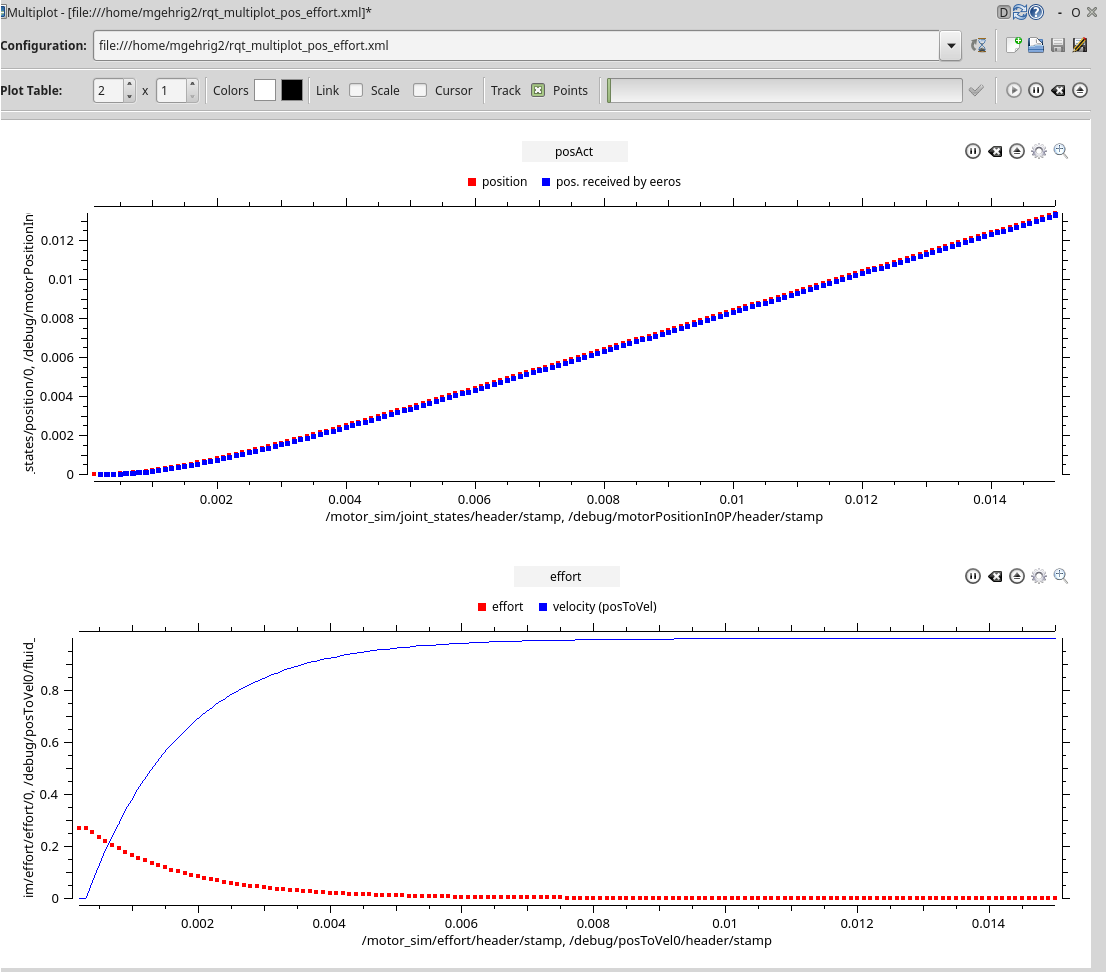
\includegraphics[angle=0,width=\textwidth]{images/motorsim_v_control_cut.png}
%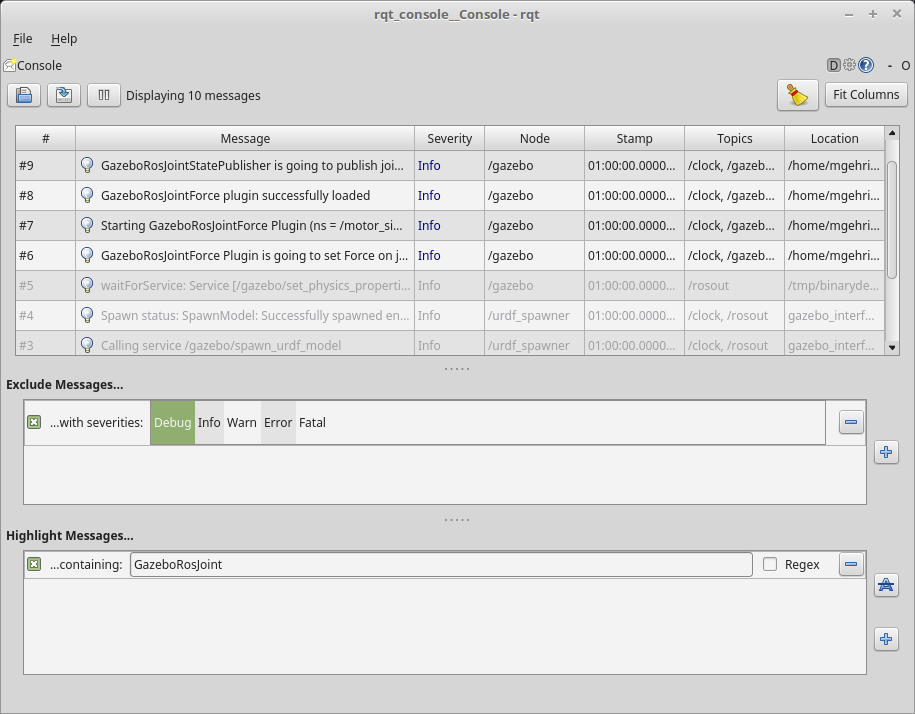
\includegraphics[angle=0,width=\textwidth]{images/screenshotRqtConsole.png}
\caption{Sprungantwort der Simulation mit Gazebo}
\label{fig:motorsim}
\end{figure}


%\textbf{Repositories:} \\
%\begin{tabular}
%  { l						| l			 							l								 l								}
%
%% Name						Repo   									Branch Aufwand     				Tag
%  EEROS\_t2.0				& \textit{Repository}: eeros-framework	& \textit{Branch}: ROSVt2		& \textit{Tag}: Test002.0 		\\
%  EEROS-Applikation\_t2.0	& \textit{Repository}: testAppVt2		& \textit{Branch}: master		& \textit{Tag}: Test002.0 		\\
%\end{tabular}
%
%\textbf{Ablauf: } \\
%\begin{enumerate}
%\item 
%%\textbf{Ergebnis:} \cmark
%\end{enumerate}
